\subsubsectionwithauthor[author={Mika Landeck},email={mika.landeck@fau.de}]{Aufgabe 2: Kontextfreie Sprachen}

\paragraph{(a)}m
	$G=(\{S,A,B\},\Sigma,P,S)$ mit $P$:\\
	\begin{tabular}{lcl}
		$S$ & $\rightarrow$ & $AB$ $\mid$ $\epsilon$ \\
		$A$ & $\rightarrow$ & $0A1 \mid 2A \mid \epsilon$ \\
		$B$ & $\rightarrow$ & $1B2 \mid B0 \mid \epsilon$ \\
	\end{tabular}
	
	\textbf{Konstruktionsidee} \\
	Im Kern beruht diese Grammatik auf der Idee, dass jedes Wort in $L$ aus zwei Teilwörtern besteht:
	\begin{itemize}
		\item
		einem linken Teilwort $x$, dass an seinem rechten Rand (also dem Mittelteil des Gesamtwortes) so viele 1en aufweist	wie es selbst 0en enthält, wobei links und rechts aller 0en beliebig viele 2en zulässig sind, und analog dazu
		\item
		einem rechten Teilwort $y$, dass an seinem linken Rand (also dem Mittelteil des Gesamtwortes) so viele 1en aufweist wie es selbst 2en enthält, wobei links und rechts der 2en beliebig viele 0en zulässig sind.			
	\end{itemize}

	Somit können $x$ und $y$ aus den Variablen $A$ und $B$ der Grammatik erzeugt werden und es ist jederzeit sichergestellt, dass im Gesamtwort $n = |w|_0 + |v|_2$ gilt, denn n entspricht der Summe der 1en in $x$ und $y$.
	
\paragraph{(b)}m 
	\underline{Ableitung:} $\underline{S}\Rightarrow \underline{A}B\Rightarrow 2\underline{A}B\Rightarrow 20\underline{A}1B\Rightarrow 202\underline{A}1B\Rightarrow 2022\underline{A}1B\Rightarrow 20221\underline{B}\Rightarrow 20221\underline{B}0\Rightarrow 202211\underline{B}20\Rightarrow 202211\underline{B}020\Rightarrow 2022111\underline{B}2020\Rightarrow 20221112020$
	
	\underline{Ableitungsbaum:}

	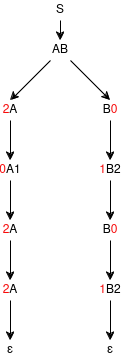
\includegraphics[scale=0.8]{Ableitungsbaum}
	
\paragraph{(c)}m
	$L = \{w1^n v \mid n \in \mathbb{N}, w, v \in \{0,2\}^*, n = |w|_0 \cdot |v|_2 \}$		
	
	\textbf{Beweis der Nicht-Kontextfreiheit}
	\begin{quote}
		\textbf{Pumpinglemma für kontextfreie Sprachen} \\
		Ist $L$ eine kontextfreie Sprache, so gilt: \\
		$\exists p \geq 1: \forall z \in L, |z| \geq p:$ \\
		$\exists u,v,w,x,y \in \Sigma^*: z = uvwxy$ mit
		\begin{enumerate}
			\item $|vx| \geq 1$
			\item $|vwx| \leq p$
			\item $\forall i \in \mathbb{N} : uv^{i}wx^{i}y \in L$
		\end{enumerate}
	\end{quote}
  	
	Nehmen wir an $L$ sei kontextfrei, dann können wir das Pumpinglemma anwenden und folgern:

	Sei $p \in \mathbb{N}$ die Pumpingzahl. Wir wählen $z = 0^p1^{p^2}2^p \in L$ mit $|z|=2p+p^2\geq p$.\\
	Aus $1$ und $2$ folgt: $vwx$ kann nicht aus $0$en, $1$en und $2$en bestehen und $vx$ darf nicht leer sein. Die Formen von $v$ und $x$ entsprechen also einem der vier Fälle (mit $1 \leq k+l+m \leq p$):
	\begin{itemize}
		\item Fall 1.1: $v=0^k1^l$ und $x=1^m$
		\item Fall 1.2: $v=0^k$ und $x=0^l1^m$
		\item Fall 2.1: $v=1^k2^l$ und $x=2^m$
		\item Fall 2.2: $v=1^k$ und $x=1^l2^m$
	\end{itemize}

	\underline{Fall 1.1:}\\
	Man erhält durch pumpen mit $i = 2$ das Wort $z'=uv^2wx^2y=0^{p+2k}1^{p^2+2(l+m)}2^{p}$.\\
	Angenommen $k\geq 1$. Damit $z' \in L$ gilt, muss $l+m = k*p$ und somit $k+l+m=k*(p+1)>p$ gelten. $\mbox{\Lightning}$\\
	Folglich muss $k=0$ sein. Aber es muss wieder $l+m = k*p = 0$ gelten und somit $k+l+m=0$. $\mbox{\Lightning}$

	\underline{Fall 1.2:}\\
	Man erhält durch pumpen mit $i = 2$ das Wort $z'=uv^2wx^2y=0^{p+2(k+l)}1^{p^2+2m}2^{p}$.\\
	Angenommen $k\geq 1$. Damit $z' \in L$ gilt, muss $m = (k+l)*p$ und somit $k+l+m=l*(p+1)+k*(p+1)>p$ gelten. $\mbox{\Lightning}$\\
	Folglich muss $k=0$ sein. Aber es muss wieder $m = (k+l)*p = l*p$ gelten.\\
	Ist nun $l\geq 1$ gilt $k+l+m=l*(p+1)>p$. $\mbox{\Lightning}$\\
	Falls aber $l=0$, ist auch $k+l+m=0$. $\mbox{\Lightning}$

	\underline{Fall 2.1:}\\
	Man erhält durch pumpen mit $i = 2$ das Wort $z'=uv^2wx^2y=0^{p}1^{p^2+2k}2^{p+2(l+m)}$.\\
	Angenommen $l\geq 1$. Damit $z' \in L$ gilt, muss $k = (l+m)*p$ und somit $k+l+m=l*(p+1)+m*(p+1)>p$ gelten. $\mbox{\Lightning}$\\
	Folglich muss $l=0$ sein. Aber es muss wieder $k = (l+m)*p = m*p$ gelten.\\
	Ist nun $m\geq 1$ gilt $k+l+m=m*(p+1)>p$. $\mbox{\Lightning}$\\
	Falls aber $m=0$, ist auch $k+l+m=0$. $\mbox{\Lightning}$

	\underline{Fall 2.2:}\\
	Man erhält durch pumpen mit $i = 2$ das Wort $z'=uv^2wx^2y=0^{p}1^{p^2+2(k+l)}2^{p+2m}$.\\
	Angenommen $m\geq 1$. Damit $z' \in L$ gilt, muss $k+l = m*p$ und somit $l+m+k=m*(p+1)>p$ gelten. $\mbox{\Lightning}$\\
	Folglich muss $m=0$ sein. Aber es muss wieder $k+l = m*p = 0$ gelten und somit $l+m+k=0$. $\mbox{\Lightning}$

	In jedem Fall ergibt sich ein Widerspruch zur Annahme $L$ sei kontextfrei. $\Rightarrow L$ ist nicht kontextfrei.
		


\newpage